\chapter{Task 28: Voter Model}

\section{Task Description}
The voter model is perhaps the simplest and most studied model of cooperative behaviour. While its behaviour on regular lattices of arbitrary dimention $d$ is known in detail, it is much more difficult to get a comprehnsive general picture of its behaviour on a complex network, where there is interplay between many factors, such as the degree distribution, the effective dimentionality, the degree of disorder, the presence of correlations \cite{suchecki_numerical}. 
The aim of this task is to describe the voter model and attempt to reproduce its behaviour on some class of networks. Specifically, I chose to focus on scale free networks, for which some analitical results have been found \cite{sood}. 

\section{Model}
In the voter model, each node of the network is in one of two possible states, say, spin up or spin down: $\sigma_i \in \{\pm 1\}$. The evolution starts with some random configuration of up and down spins. The update rule is defined as follows: 
\medskip
\newline
\begin{minipage}{0.8\textwidth}
\begin{itemize}
    \item[i)] choose one node at random,
    \item[ii)] choose one of its neighbors at random,
    \item[iii)] ascribe to this node the current state of its neighbour.
\end{itemize}
\end{minipage}
\hfill
\begin{minipage}{0.2\textwidth}
\vfill
    \textit{Node-update rule}
\vfill
\end{minipage}
\medskip
\newline
Actually, there is an alternative rule which may look equivalent:
\medskip
\newline
\begin{minipage}{0.8\textwidth}
\begin{itemize}
    \item[i)] choose one link at random,
    \item[ii)] choose one of its ends at random,
    \item[iii)] ascribe to this node the current state of the other end.
\end{itemize}
\end{minipage}
\hfill
\begin{minipage}{0.2\textwidth}
\vfill
    \textit{Link-update rule}
\vfill
\end{minipage}
\medskip
\newline
Indeed the two rules are equivalent for regular lattices, but not in the case of complex networks \cite{suchecki_analitical}. For each time step, this update rule is applied $N$ times if $N$ is the network size, so that \textit{on average} each node is updated once. The voter model defines a markovian stochastic process. There are two absorbing states: all spins up and all spins down (when it reaches one of these states, it cannot change anymore, that is why they are called absorbing). If we identify network nodes as people and spin up and down with two possible opinion, the absorbing state represent consensum. \\
There is always a chance that a finite size network reaches consensus. In fact, \textbf{the mean time to reach consensus in a finite network is always finite} (the mean is here intended over the set of all evolution histories and initial conditions), whether it is a regular lattice or a complex network. However, conceptually there are different scenarios when infinite size networks are considered instead.\\
The mean time $\<\tau\>$ to reach consensus in a finite, regular lattice of $N$ nodes and dimention $d$ is known to scale as:
\begin{equation*}
    \<\tau\>(N) \sim
    \begin{cases}
        N^2 \quad &\text{if}\quad d=1 \\
        N\cdot \ln{N} &\text{if}\quad d=2 \\
        N &\text{if}\quad d>2 \\
    \end{cases}
\end{equation*}
For networks, one could guess to find $\<\tau\>(N) \sim N$ as for high dimentional lattices. However this is not true in general. For instance, \cite{sood} found analitically that, for uncorrelated, scale-free networks with degree distribution $P(k)\sim k^{-\gamma}$ and \textit{node-update} rule:
\begin{equation*}
    \<\tau\>(N) \sim
        \begin{cases}
         N^{\alpha}, \, \alpha<1 \quad &\text{if}\quad \gamma < 3 \\
        \frac{N}{\ln{N}} &\text{if}\quad \gamma = 3 \\
         N &\text{if}\quad \gamma > 3 \\
    \end{cases}
\end{equation*}
Generically, $\tau(N)$ grows sublinearly with N; that is, high-degree nodes greatly accelerate the approach to consensus. \cite{suchecki_numerical} numerically found for Barabasi-Albert networks a scaling $\tau \sim N^{0.88}$, which is compatible with $\tau \sim \frac{N}{\ln{N}}$, and a scaling $\tau \sim N$ (like for the high dimentional lattices) when the \textit{edge-update} rule is used instead. \\
A standard order parameter used to measure the ordering process of the voter dynamic is the \textit{average interface density $\rho$}, defined as the density of edges connecting nodes with different states:
\begin{equation}
    \rho(\mathbf{\sigma}) := \frac{\sum_{i,\,j}\left[A_{i,\,j}\,\cdot \mathbbm{1}(\sigma_i,\,\sigma_j)\right]}{\sum_{i,\,j}\, A_{i,\,j}}, \quad \text{where} \, \mathbbm{1}(\sigma_i,\,\sigma_j):= \frac{1 - \sigma_i\,\sigma_j}{2} = 
    \begin{cases}
        1 & \text{if}\quad \sigma_i\neq \sigma_j \\
        0 & \text{if}\quad \sigma_i= \sigma_j \\
    \end{cases}
\end{equation}
\section{Simulation results}
\begin{figure}[H]
    \centering
    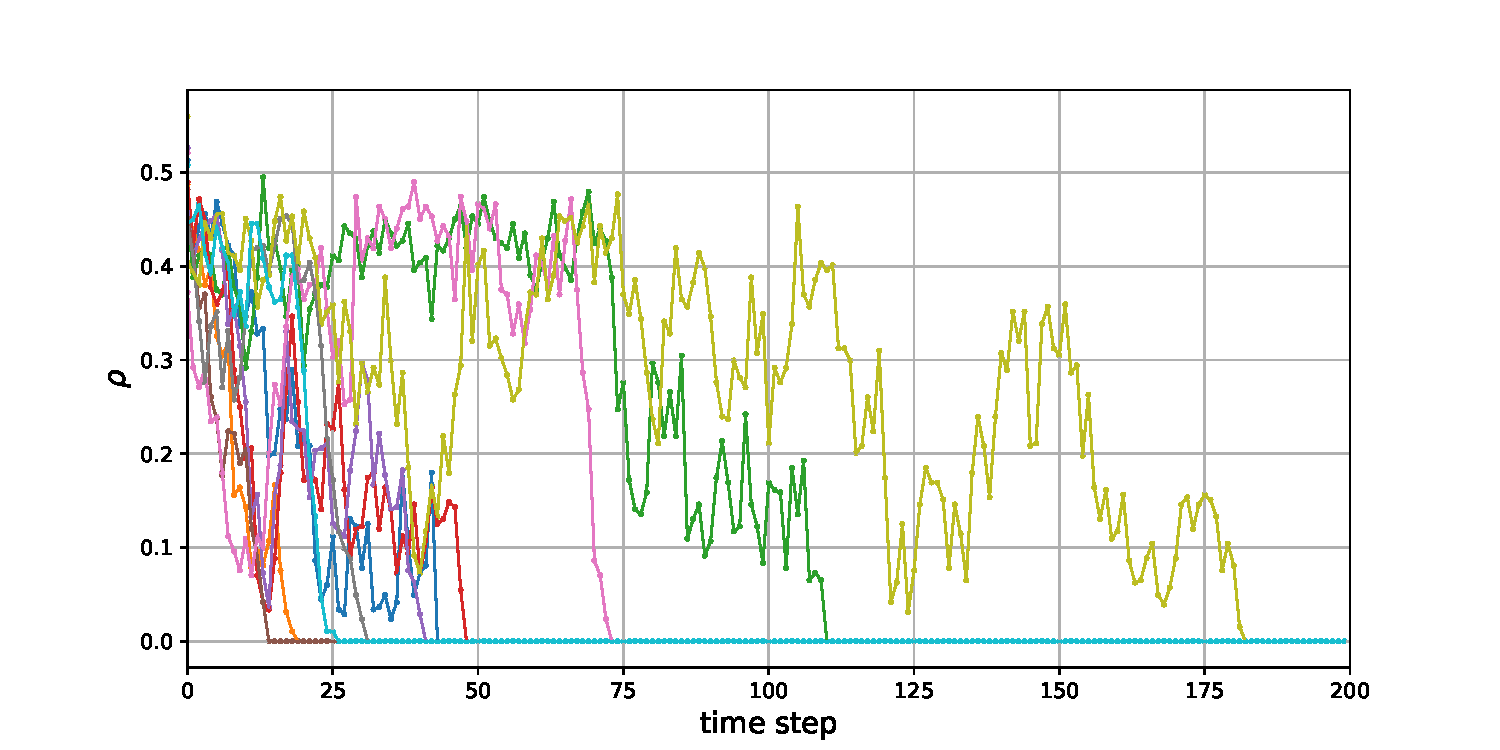
\includegraphics[width=\linewidth]{latex_source/images/voter/example_evolution.pdf}
    \caption{Evolution of the voter model on Barabasi-Albert networks with $N=100$ and $\<k\> = 8$. Each line is a trajectory on a different network instance of the BA model. Initial state is drawn uniformly at random for each trajectory.}
    \label{fig:enter-label}
\end{figure}

\begin{figure}[H]
    \centering
    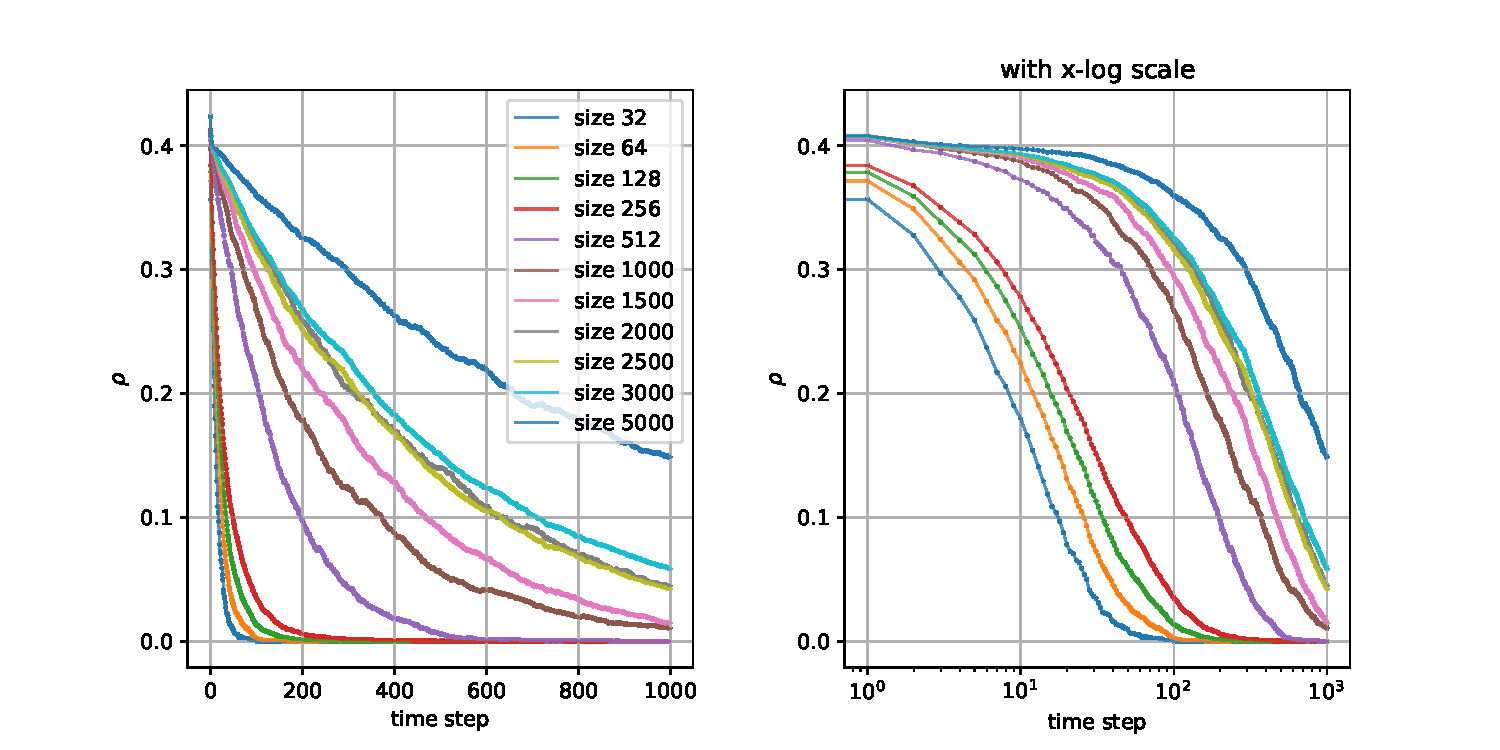
\includegraphics[width=\linewidth]{latex_source/images/voter/BA_node_update_rule_results_logscale.pdf}
    \caption{Evolution of the average interface density [Eq. $\ref{eq:rho}$] in Barabasi Albert networks of different sizes (see legend) and mean degree $\<k\>= 6$. Data is averaged over $500$ realizations. }
    \label{fig:BA_evolution}
\end{figure}

\begin{figure}[H]
    \centering
    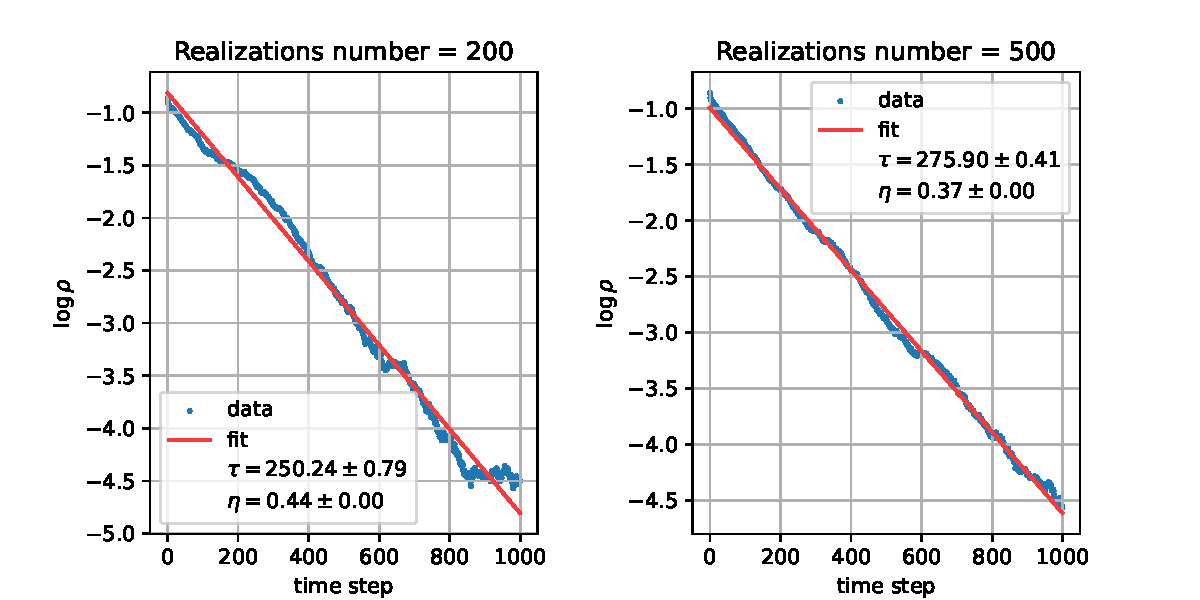
\includegraphics[width=\linewidth]{latex_source/images/voter/comparison.pdf}
    \caption{Comparison between exponential fit parameters estimated from $200$ (left) and $500$ (right) different realization on BA networks with same size $N=1000$. }
    \label{fig:enter-label}
\end{figure}

\begin{figure}[H]
    \centering
    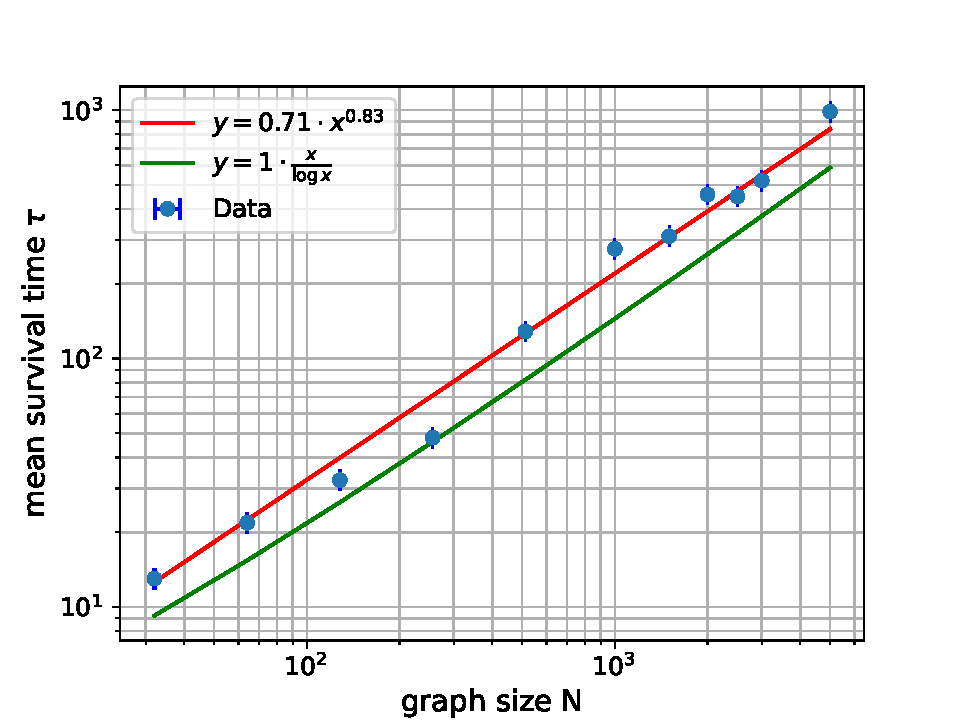
\includegraphics[width=\linewidth]{latex_source/images/voter/BA_time_scaling.pdf}
    \caption{Average survival times for Barabasi Albert networks of different sizes, as results from the exponential fit of the curves in [Fig: $\ref{fig:BA_evolution}$]. Data is fitted with a power law $y = \alpha \cdot x^\gamma$ with free parameters $\alpha,\, \gamma$ with the method of least squares implemented in \textbf{scipy.optimize.curve\_fit} from Phyton library Scipy \cite{scipy}. The best estimation for fit parameters are $\gamma = 0.8312 +/- 0.0007$, $\alpha = 0.707 +- 0.004$. The fit curve is \textcolor{red}{red}. For comparison, also the theoretical expectation $\tau \sim \frac{N}{\log{N}}$ is plotted. One can see that the slope of the two curves are very similiar. To make $x/logx$ fit the data, one simply needs to add a prefactor, which corresponds to an intercept in the log log scale of the plot presented here.}
    \label{fig:BA_scaling}
\end{figure}